\documentclass{beamer}
\usepackage[utf8]{inputenc}
\usepackage{braket}
\usepackage{mathtools}
\usetheme{Berlin}
\title{Notas de mecánica y computación cuántica}
\author{Gabriel Acosta}

\begin{document}
\begin{frame}
  \titlepage
\end{frame}

\begin{frame}
  \frametitle{Qubits}
  Justo como en computación clásica el bit es el concepto fundamental con el que se describe la información,
  existe un análogo al mismo en computación cuántica.: el bit cuántico o \textit{qubit}
  
\end{frame}

\begin{frame}
  \frametitle{Qubits}
  Podemos tratar en un principio a los qubits como objetos matemáticos con un \textit{estado} que lo describe.
  Así como computación clásica el estado de un bit puede ser representado por medio de \textit{0} o
  \textit{1}, dos posibles estados pueden describir a un qubit: $\ket{0}$ o $\ket{1}$
\end{frame}

\begin{frame}
  \frametitle{Superposición}
  Se pueden formar una combinación lineal de los estados de un qubit, llamado \textit{superposición}:
  

  $$\ket{\Psi} = \alpha\ket{0} + \beta\ket{1}$$

  Donde $\alpha$ y $\beta$ son números complejos.
  En otras palabras, un qubit es un espacio vectorial de dos elementos.
  Los estados $\ket{0}$ y $\ket{1}$ son los \textit{estados base computacionales} y forman
  una base ortornormal para este espacio vectorial.

  
\end{frame}

\begin{frame}
  \frametitle{Observación}
  No es posible examinar un qubit en busca del estado exacto en que se encuentra, es decir obtener los valores
  $\alpha$ y $\beta$. En cambio, al \textit{medir} un qubit haremos colapsarlos a uno de sus estados.
  Podremos obtener 0, con una probabilidad de $|\alpha|^{2}$; o ,en su defecto, 1 con una probabilidad  de
  $|\beta|^{2}$.
  Debe cumplirse que $|\alpha|^{2} + |\beta|^{2} = 1$.
\end{frame}

\begin{frame}
  \frametitle{Esfera de Blosch}
  La esfera de Bloch es una representación geométrica del espacio de estados puros de un sistema cuántico de dos niveles.
      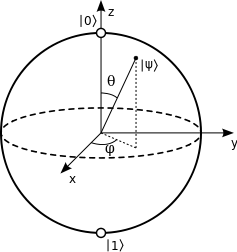
\includegraphics[scale=.60]{blochsphere.png}
\end{frame}

\begin{frame}
  \frametitle{Compuertas de un solo qubit}
  A diferencia de la computación clásica, donde solo existe una compuerta lógica no trivial de un solo bit (NOT),
  en computación cuántica existe más de una.
\end{frame}

\begin{frame}
  \frametitle{Compuerta NOT}
  Sea 
  $$\ket{\Psi} = \alpha\ket{0} + \beta\ket{1}$$
  al aplicar la compuerta NOT sobre los estados sucede que
  $$\ket{\Psi} = \alpha\ket{1} + \beta\ket{0}$$
  De manera que la compuerta actúa de manera lineal sobre el sistema.
\end{frame}

\begin{frame}
  \frametitle{Compuerta NOT}
  Así, es conveniente representar la compuerta NOT cuántica como una matriz.
  $$X \equiv
  \begin{pmatrix}
    1 & 0 \\
    0 & 1
  \end{pmatrix}$$
  
  
\end{frame}

\begin{frame}
  Si escribimos $\alpha\ket{1} + \beta\ket{0}$ usando notación de vectores
  $$
  \begin{bmatrix}
    \alpha \\
    \beta
  \end{bmatrix}
  $$

  Entonces, la compuerta NOT actuando sobre el sistema y su respectiva salida es:

  $$
  X\begin{bmatrix}
    \alpha \\
    \beta
  \end{bmatrix} =
  \begin{bmatrix}
    \beta \\
    \alpha
  \end{bmatrix}
  $$
\end{frame}

\begin{frame}
  \frametitle{Esfera Blosch de X}
  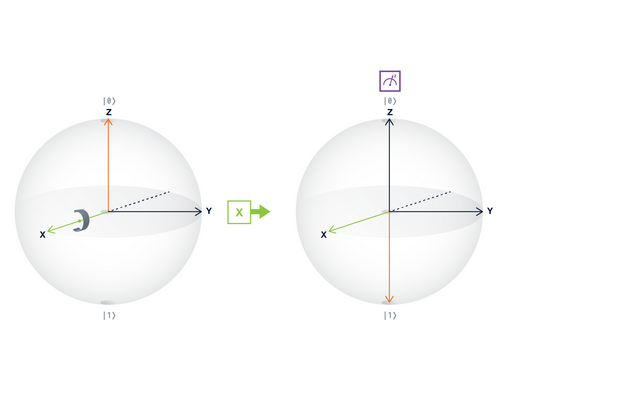
\includegraphics[scale=.60]{x-blochsphere.png}
\end{frame}

\begin{frame}
  \frametitle{Circuito de la plataforma de IBM para X}
  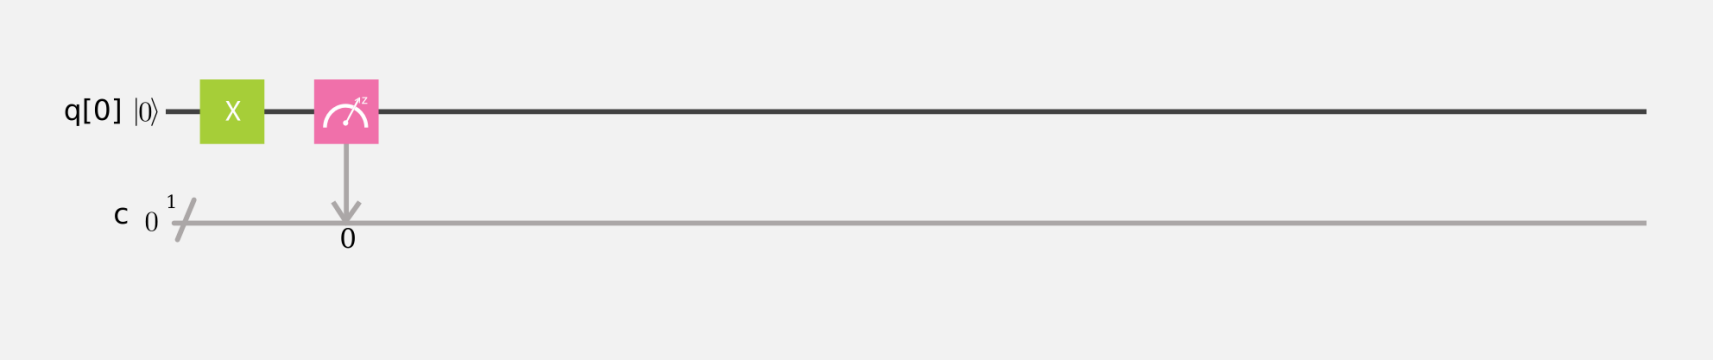
\includegraphics[scale=.15]{x-gate.png}
\end{frame}


\begin{frame}
  \frametitle{Resultado de la plataforma de IBM para X}
  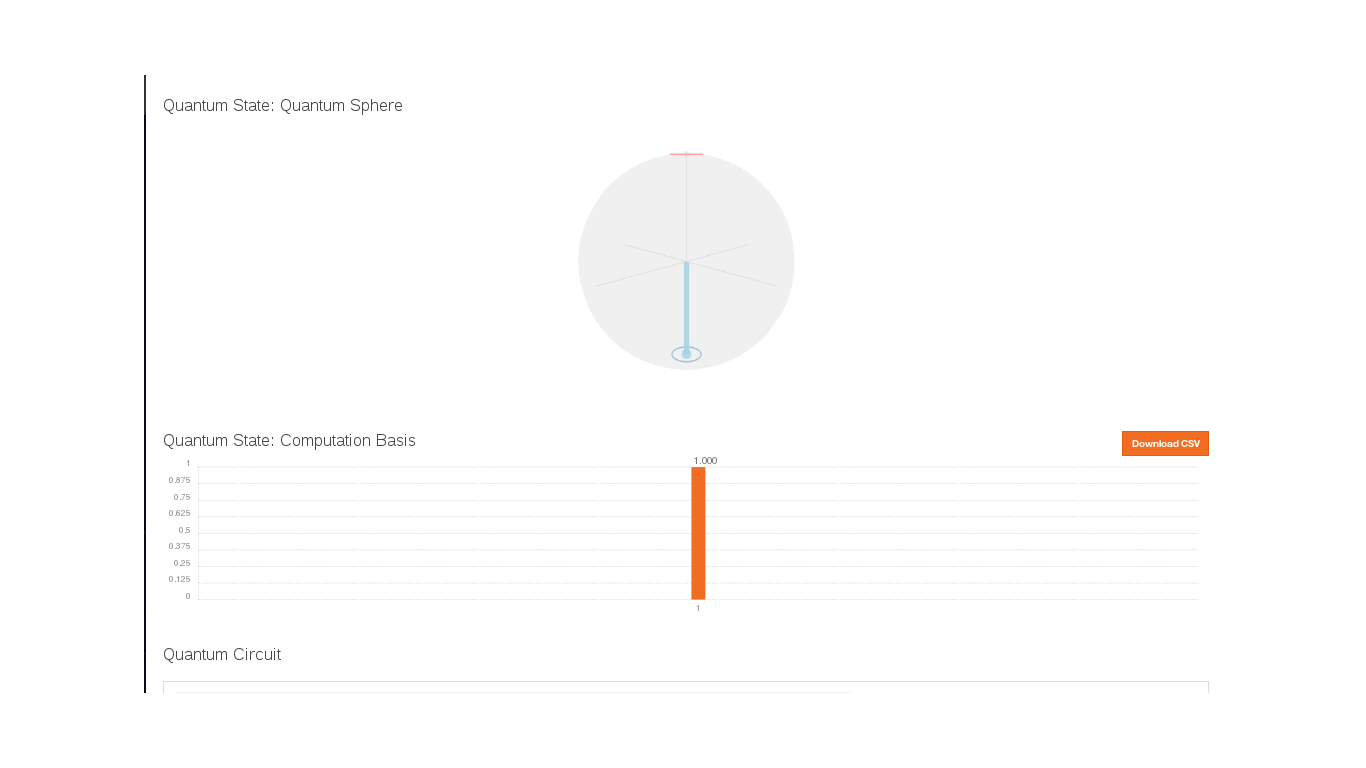
\includegraphics[scale=.30]{x-resultado.png}
\end{frame}

\begin{frame}
  \frametitle{Creando superposiciones}
  Ahora que se ha abordado como cambiar entre los estados $\ket{0}$ y $\ket{1}$, podemos explorar el concepto de
  superposición; se refiere a crear un nuevo estado cuántico el cual es una combinación lineal de los estados base
  $\ket{0}$ y $\ket{1}$.
\end{frame}

\begin{frame}
  \frametitle{La compuerta Hadamard \textit{H}}
  La compuerta Hadamard es descrita con la siguiente matriz
    $$H \equiv
  \frac{1}{\sqrt{2}}\begin{pmatrix}
    1 & 1 \\
    1 & -1
  \end{pmatrix}$$
\end{frame}

\begin{frame}
  Si ahora hacemos pasar el estado $\ket{0}$ a través de la compuerta H, tenemos como resultado:
  $$ \ket{+} = \frac{1}{\sqrt{2}}( \ket{0} + \ket{1} ) $$
  $\ket{+}$ puede decirse que está 'a la mitad del estado $\ket{0}$ y a la mitad del
  $\ket{1}$', lo cuál es una clara \textit{superposición de estados}.
\end{frame}

\begin{frame}
  Ahora bien, hacemos pasar a $\ket{1}$ través de la compuerta \textit{H}, dando como
  resultado:
  $$ \ket{-} = \frac{1}{\sqrt{2}}( \ket{0} - \ket{1} ) $$
  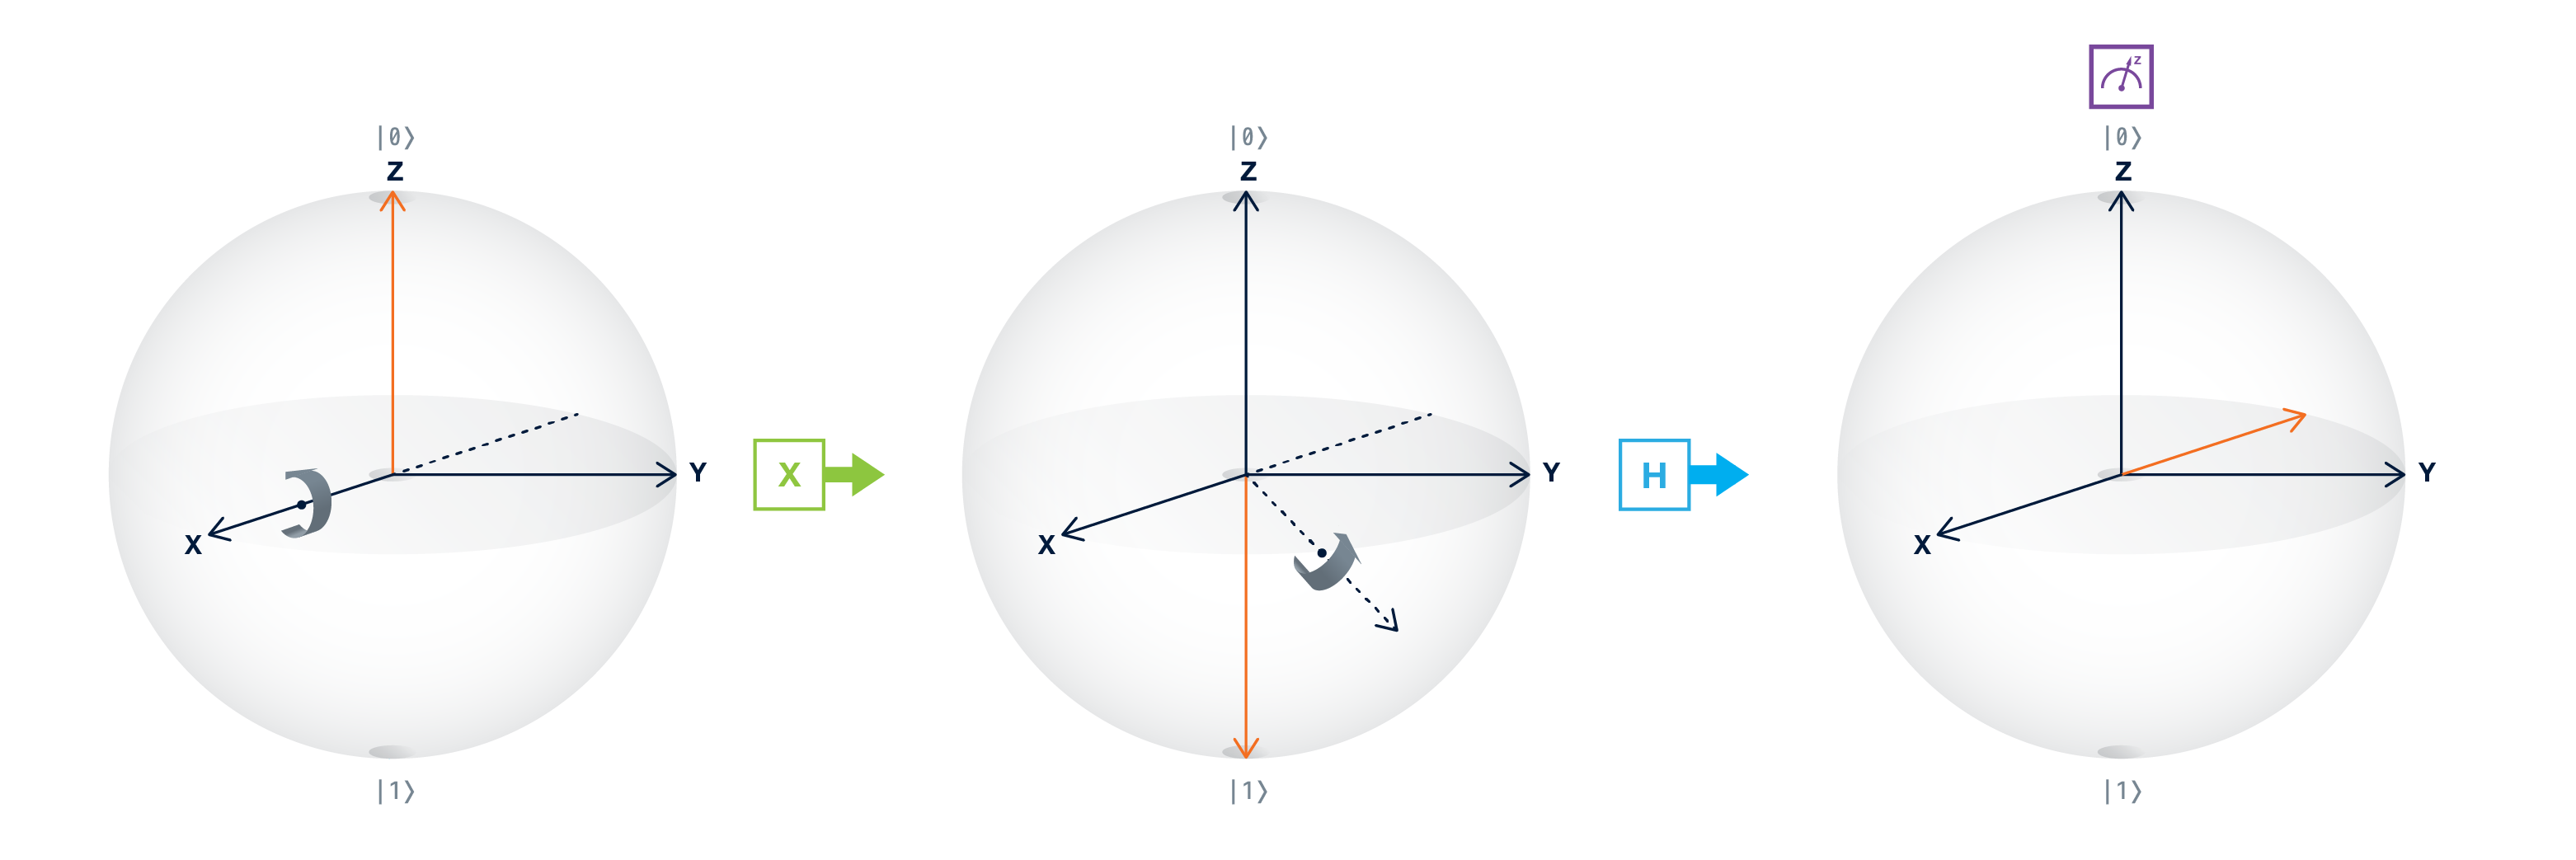
\includegraphics[scale=.2]{-superpositionstate.png}
\end{frame}
\begin{frame}
  $\ket{+}$ y $\ket{-}$ forman así mismo una nueva base computacional (o una nueva dirección de
  medición), llamada la base de superposición.
\end{frame}

\begin{frame}
  Se puede observar a la compuerta \textit{H} como un intercambio en los ejes X+Z

  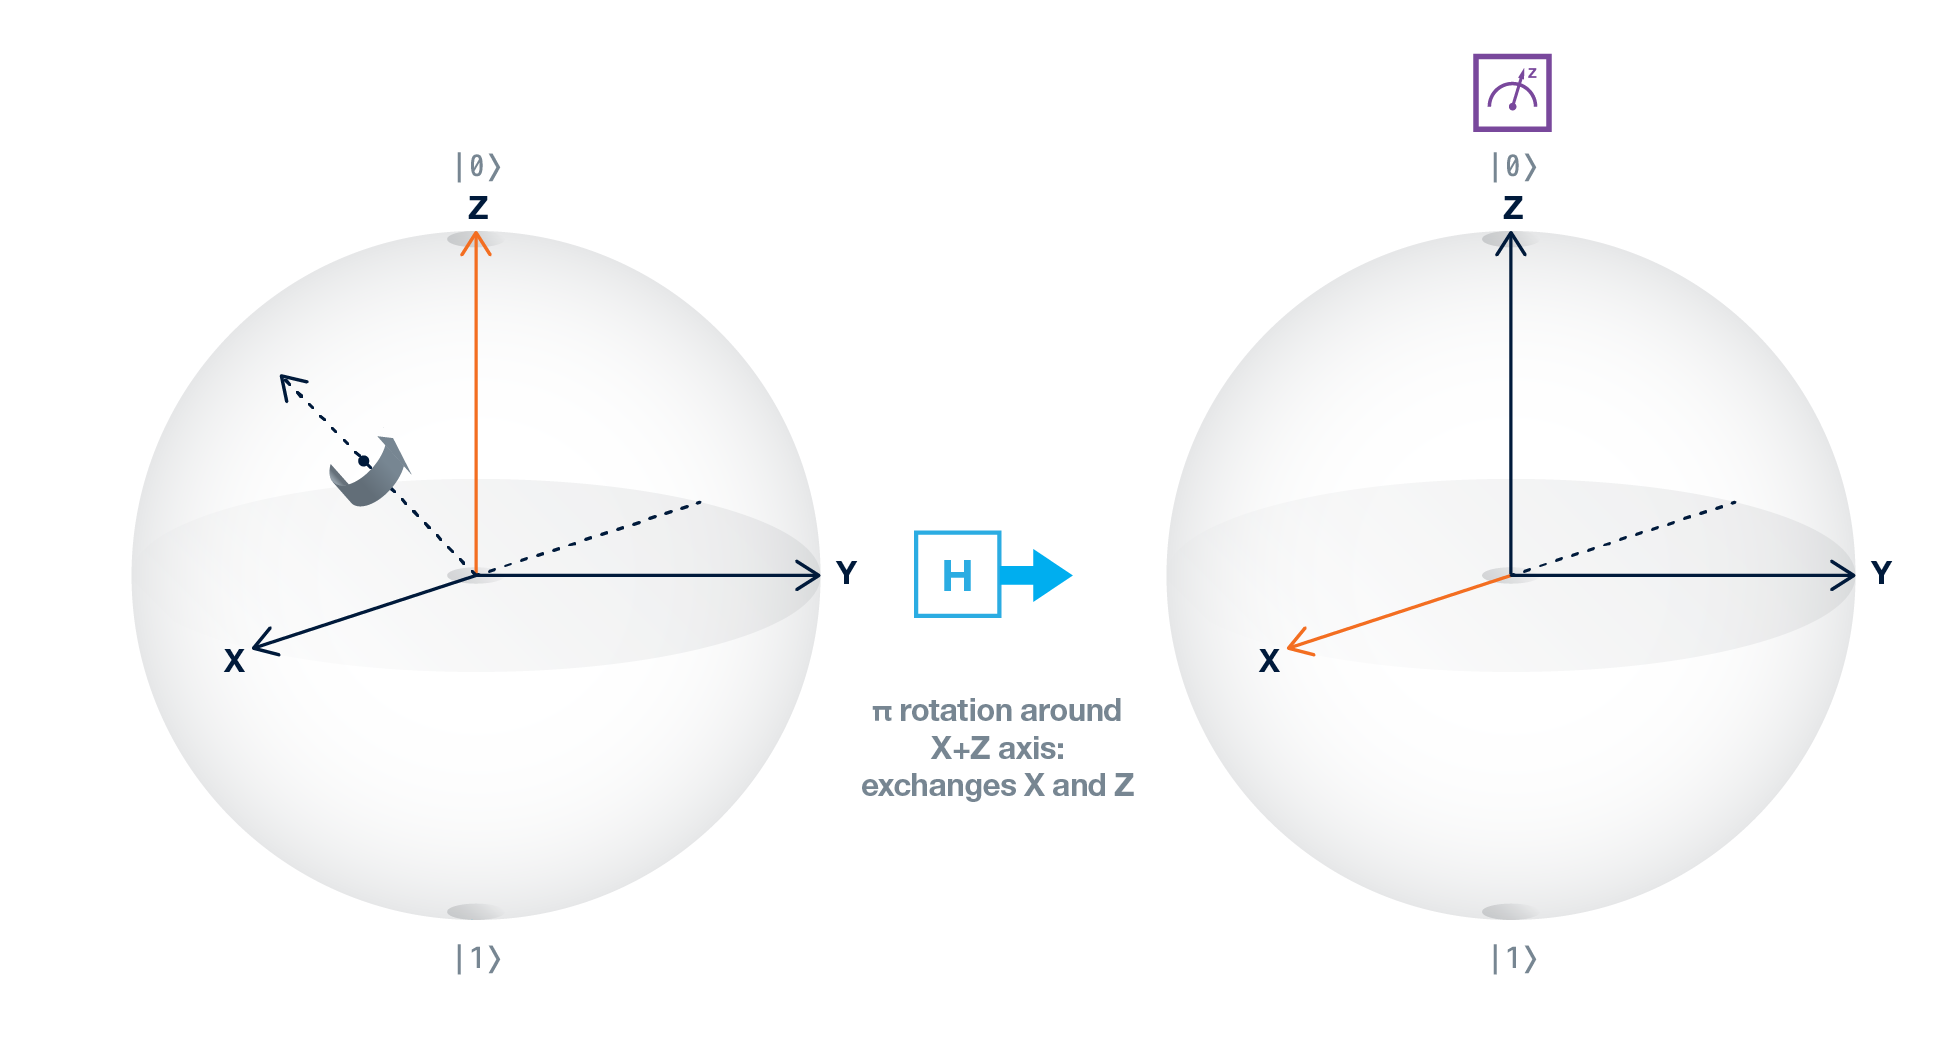
\includegraphics[scale=.3]{HADAMARD-GATE-BLOSCH.png}
\end{frame}

\begin{frame}
  \frametitle{Experimento con la CNOT en la plataforam de IBM}
  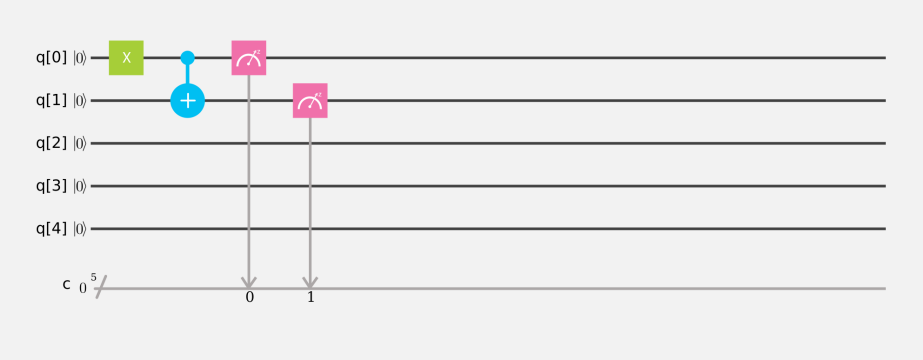
\includegraphics[scale=.35]{CNOT-IBM-CIRCUIT.png}
\end{frame}

\begin{frame}
  \frametitle{Resultados}
  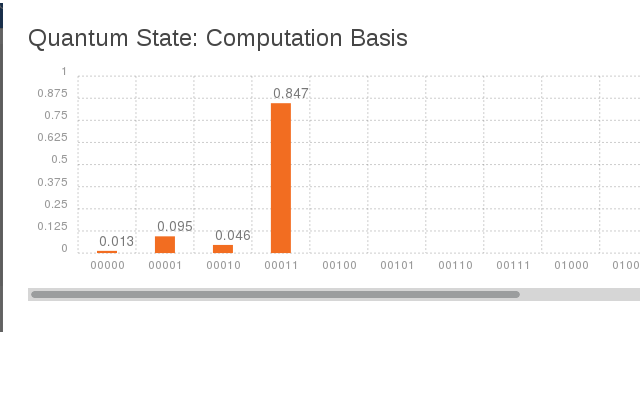
\includegraphics[scale=.5]{CNOT-RESULTADOS.png}
\end{frame}

\end{document}
